\chapter{Intermediate Representation (IR) Model}
\label{ch:ir_formalization}

\section{Introduction}
The proposed analysis process is configured as a pipeline of
functional transformations. Given a source code $S$ belonging to a
language $L \in \{C, C++, Java, Python, Rust\}$, the system generates
an abstract Component Tree through an extraction function $E: CST_L
\to IR$. The goal of the IR is to provide a domain $\mathcal{D}_{IR}$
that is a \textit{conservative extension}
\cite{TODO:conservative_extension} of the high-level syntactic
constructs, guaranteeing Type
Safety in the subsequent dependency resolution phase $R: IR \to
\mathcal{G}$, where $\mathcal{G}$ is the dependency graph.

Formally, we define the \textbf{Intermediate Representation Domain}
$\mathcal{D}_{IR}$ as the space of all possible valid
\textit{Component Trees}. Each instance $T \in \mathcal{D}_{IR}$
corresponds to the root of a hierarchy of components (represented by
the Module type $\mathcal{M}$, defined below) that recursively
aggregates the entire structure of the analyzed software.

\section{The Type System $\mathcal{T}$}
To ensure language agnosticism, we define the type system as an
algebra of sum and product types \cite{TODO:algebraic_data_types}.

\subsection{Identifiers and Paths ($\pi$)}
Let $\mathcal{I}$ be the set of valid strings as identifiers. We
define the type \textbf{Qualified Name} ($\pi$) as the set of finite
non-empty sequences of identifiers:
$$\pi = \{ \langle \iota_1, \iota_2, \dots, \iota_n \rangle \mid
\iota_j \in \mathcal{I}, n \geq 1 \}$$
This type uniquely maps namespaces, Java packages, Rust modules, and
resolved scopes in C++.

\subsection{Type References ($\tau$)}
A type reference $\tau$ in the IR models the lifecycle of symbol
discovery and resolution. To guarantee \textit{Type Safety} between
the extraction phases and the graph generation, we define $\tau$ as
an eight-state sum type:
\begin{align*}
  \tau ::=&\ \text{Prim}(\mathcal{T}_{p}) \\
  &\mid \text{Unresolved}(\pi_{raw}) \\
  &\mid \text{ResolutionQuery}(\mathcal{Q}) \\
  &\mid \text{Resolved}(\pi_{abs}) \\
  &\mid \text{External}(\pi_{ext}) \\
  &\mid \text{Union}(\vec{\tau}) \\
  &\mid \text{EvaluatedAccess}(\tau_{path}, \tau_{type}) \\
  &\mid \text{Failed}(\pi_{raw})
\end{align*}
Where:
\begin{itemize}
  \item \textbf{Prim}: Represents fundamental primitive types
    ($\mathcal{T}_{p}$). Since primitive keywords vary drastically
    across languages, the set $\mathcal{T}_{p}$ is not static but
    provided by a Data-Driven architectural \textit{Primitive
    Registry} populated at load time. Being defined at the language
    level, they do not require resolution.
  \item \textbf{Unresolved}: A raw text path extracted by the parser
    before any substitution.
  \item \textbf{ResolutionQuery($\mathcal{Q}$)}: Represents an
    algebraic expression composed of \texttt{Find}, \texttt{Extract},
    and \texttt{Call} operations. It is the partial product that
    defers resolution to Phase 2.
  \item \textbf{Resolved}: Represents a user-defined type (internal
    to the project) whose declaration or definition has been
    successfully localized and associated within the absolute
    namespace of the project. The path $\pi_{abs}$ is relative to the
    root of the module tree.
  \item \textbf{External}: Represents a type that is recognized and
    spatially localized, but belongs to a module or ecosystem outside
    the provided source code (e.g., standard libraries,
    \texttt{java.util.*}, external crates).
  \item \textbf{Union($\vec{\tau}$)}: Captures a disjunction of types
    (e.g., \texttt{Union[A, B]} in Python or \texttt{A | B} in
    TypeScript). It maintains a vector of references that must be
    individually processed.
  \item \textbf{EvaluatedAccess($\tau_{path}, \tau_{type}$)}: A
    wrapper that preserves both the originally queried path and the
    final structural type. This ensures that intermediate access
    chains generate corresponding dependency edges.
  \item \textbf{Failed($\pi_{raw}$)}: Indicates that the static
    resolution phase has failed. It keeps track of the target path to
    support fallback analysis and calculate statistical metrics on
    \textit{Recall} (coverage and confidence of the analyzer).
\end{itemize}

Figure \ref{fig:typeref_lifecycle} illustrates the complete state
machine of a type reference during the analysis pipeline. This
rigorous separation allows the type system to enforce that graph
generation occurs exclusively from \texttt{Resolved} or
\texttt{External} references.

\begin{figure}[htpb]
  \centering
  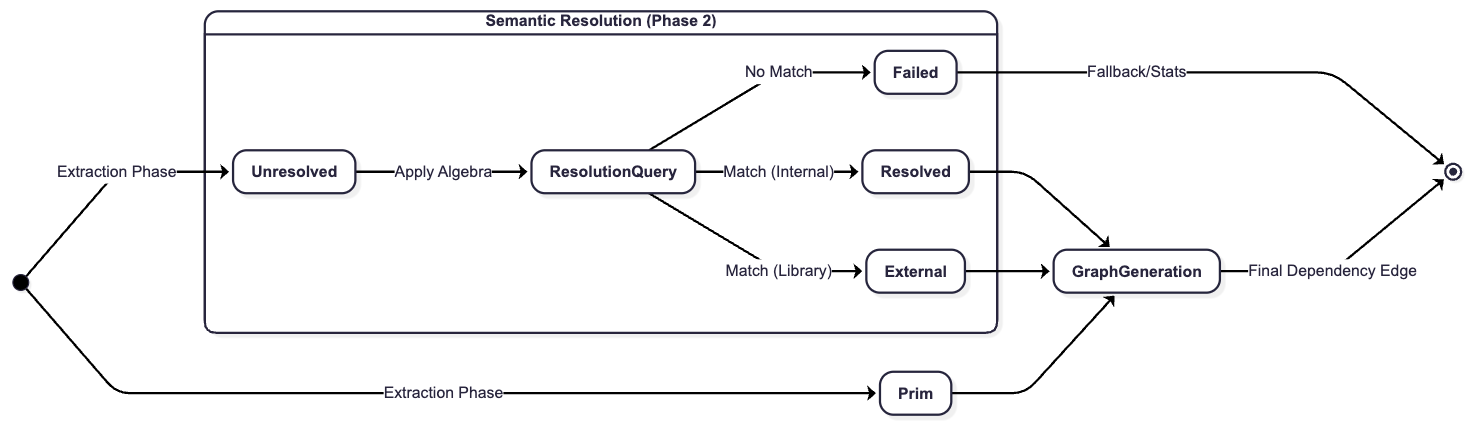
\includegraphics[width=0.8\textwidth]{images/typeref_lifecycle.png}
  \caption{State machine diagram illustrating the lifecycle of a Type
  Reference ($\tau$) from syntactic extraction to semantic resolution.}
  \label{fig:typeref_lifecycle}
\end{figure}

\section{Modeling Structural Constructs}
Structured Types represent the core of the architectural analysis.
They are modeled as product types whose components define the state
and behavior of the entity.

\subsection{Members and Signatures}
We define the \textbf{Field} type ($f$), representing an attribute or
data field, defined as the product of an identifier, a type
reference, and a set of associated annotations/decorators:
$$f = \iota \times \tau \times \mathcal{P}(\tau)$$
We define the \textbf{Parameter} type ($p$) to handle parameters
passed to functions:
$$p = \iota^? \times \tau \times \mathbb{B}$$ where the identifier
$\iota^?$ is optional (to support lambda functions and anonymous
parameters), $\tau$ is the type, and $\mathbb{B}$ indicates the
variadic property of the parameter.

To abstract the concept of a function's "signature" from the
component that implements it, we introduce the \textbf{Signature}
type ($\sigma$):
$$\sigma = \vec{p} \times \tau_{ret}$$
where $\vec{p}$ is the parameter vector and $\tau_{ret}$ is the return type.

Building on this, to model the hierarchical body of a function, we
introduce the \textbf{Block} construct ($\mathcal{B}$). A lexical
block (typically delimited by braces \texttt{\{\}}) isolates an
internal scope where local variables can be declared. Leveraging the
same structure as data fields ($f = \iota \times \tau$), local
variables are elegantly formalized as a vector of $f$. The block
tracks its behavioral dependencies and can recursively nest further
blocks (as in \texttt{if} or \texttt{while} statements):
$$\mathcal{B} = \langle \vec{f}_{local}, \vec{\tau}_{calls},
\vec{\tau}_{inst}, \vec{\tau}_{accesses}, \vec{\tau}_{casts},
\vec{\mathcal{B}}_{sub} \rangle$$
where $\vec{\tau}_{calls}$ represents the set of type references
whose functions are explicitly invoked within the block,
$\vec{\tau}_{inst}$ represents the structured types explicitly
instantiated (e.g., via \texttt{new}), $\vec{\tau}_{accesses}$
represents the direct read or write references to a component's
state, and $\vec{\tau}_{casts}$ captures explicit type casts (e.g.,
\texttt{as} conversions or C-like casts).

Finally, we define the universal \textbf{Function} type
($\mathcal{F}$) as a container that binds a qualified name to a
specific signature, an optional root block modeling its body, a
boolean flag for constructors, and a set of annotations:
$$\mathcal{F} = \langle \pi, \sigma, \mathcal{B}^?,
\mathbb{B}_{ctor}, \mathcal{P}(\tau) \rangle$$

The architectural role of an $\mathcal{F}$ (whether it acts as a
Method or a Free Function) is not encoded in its type, but is
determined exclusively by the structural context in which it is
placed (within a structured type or a module).

Overloading is naturally handled by the cardinality of the set of
functions within a structured type or module: an entity can contain
multiple functions with the same $\mathcal{I}$ but different
signatures $\sigma$.

\subsection{Structured Types ($\mathcal{S}$)}
Let $\mathcal{K} = \{ \text{Class, Struct, Interface, Trait, Enum,
EnumVariant} \}$ be the domain of structured type categories. A
structured type is defined by the tuple:
$$\mathcal{S} = \langle \pi, k \in \mathcal{K}, \vec{f},
\vec{\mathcal{F}}, \vec{\tau}_{sup}, \vec{\mathcal{S}}_{nest},
\mathcal{P}(\tau), \vec{\delta}_{imp} \rangle$$
where:
\begin{itemize}
  \item $\pi$: the unique name identifying the entity within the system.
  \item $k$: the structural category (defined in $\mathcal{K}$) that
    preserves the original semantics of the construct.
  \item $\vec{f}$: the set of fields that compose the state of the entity.
  \item $\vec{\mathcal{F}}$: the set of functions (assuming the role
    of methods) that define the behavior of the entity.
  \item $\vec{\tau}_{sup}$: the set of references to super-types,
    modeling inheritance or trait/interface implementation relationships.
  \item $\vec{\mathcal{S}}_{nest}$: the set of nested types.
  \item $\mathcal{P}(\tau)$: the set of annotations, attributes, or
    decorators applied to the entity.
  \item $\vec{\delta}_{imp}$: the set of explicit dependencies
    (imports) defined within the scope of the structured type.
\end{itemize}

\subsection{Type Alias ($\mathcal{A}$)}
A \textbf{Type Alias} allows defining a new name for an existing
type. It is modeled as the tuple:
$$\mathcal{A} = \langle \pi, \tau_{target} \rangle$$
where $\tau_{target}$ is the reference to the original type. During
graph construction, they are maintained as independent nodes to
accurately track the semantic use of domains.

\subsection{Implementation Extensions ($\mathcal{X}$)}
To support languages like Rust and C++ (separation between
declaration and definition), during extraction we introduce the
temporary construct \textbf{ImplBlock} or \textbf{Implementation Extension}:
$$\mathcal{X} = \langle \pi, \tau_{target}, \tau_{trait}^?,
\vec{\mathcal{F}}, \vec{\mathcal{S}}_{nest}, \vec{\mathcal{A}} \rangle$$
where $\pi$ is the name of the extension (usually derived from the
target), $\tau_{target}$ is the type to which the implementation
applies, $\tau_{trait}^?$ is an optional reference to the implemented
trait or interface, and the other fields represent functions, nested
types, and aliases associated with the extension.
As processed in the Resolution Phase (Phase 1 and 2), extensions act
as "syntactic sugar": their methods, nested types, and traits are
\textit{flattened} into the reference structured type, effectively
disappearing from the final unified architectural model.

\section{Component Architecture}
Once analyzed, the entire software system is represented as an
instance of the \textbf{Module} type ($\mathcal{M}$), which serves as
the root of the \textit{Component Tree}. Every element $T \in
\mathcal{M}$ represents a hierarchical forest of components,
recursively aggregating the entire software structure (nested
modules, structured types, and functions). This structure constitutes
the domain of our intermediate representation.

\subsection{Component ($\mathcal{C}$)}
We define a \textbf{Component} ($\mathcal{C}$) as the disjoint union
(sum type) of the definitive structural constructs of the system.
Each component represents the logical unit that can appear as a
vertex in the dependency graph:
$$\mathcal{C} ::= \text{Mod}(\mathcal{M}) \mid
\text{StructuredType}(\mathcal{S}) \mid \text{TypeAlias}(\mathcal{A})
\mid \text{Function}(\mathcal{F}) \mid \text{Field}(\pi, \tau) \mid
\text{Primitive}(str) \mid \text{External}(\pi)$$

\subsection{Module ($\mathcal{M}$)}
The entire program structure is captured by the \textbf{Module} type
($\mathcal{M}$), defined recursively to reflect the hierarchy of the
file system or namespaces:
$$\mathcal{M} = \langle \pi, str_{lang}^?, str_{path}^?,
\vec{\delta}_{imp}, \vec{\mathcal{M}}_{nest}, \vec{\mathcal{S}},
\vec{\mathcal{A}}, \vec{\mathcal{F}}, \vec{f}_{free},
\vec{\mathcal{X}} \rangle$$
where $\vec{\delta}_{imp}$ is the set of explicit dependencies
(import/use/include) defined in the module. Each element
$\delta_{imp}$ contains the base path, an optional alias, and a flag
indicating a \textit{wildcard} inclusion. Every software element is
therefore a node in a component tree $T \in \mathcal{D}_{IR}$.

A complete overview of the entities described so far, their
composition, and their semantic references is illustrated in Figure
\ref{fig:ir_model} via a UML class diagram.

\begin{figure}[htpb]
  \centering
  
\includegraphics[width=\textwidth]{images/IR_model.png}
  \caption{UML class diagram representing the complete Intermediate
    Representation (IR) domain model, highlighting hierarchical
  composition and semantic references via \texttt{TypeRef}.}
  \label{fig:ir_model}
\end{figure}

\section{Analyzer Configuration ($\mathcal{K}_{cfg}$)}
To guarantee flexibility in adapting to different linguistic
ecosystems and the diverse precisions required, the analyzer supports
a parametric configuration model:
$$\mathcal{K}_{cfg} = \langle \text{ModuleConfig},
\text{TransitiveImports}, \text{SupportImplBlocks}, \text{SelfKeyword} \rangle$$
where:
\begin{itemize}
  \item \textbf{ModuleStrategies} models logical grouping rules and
    is composed of a tuple of orthogonal boolean flags: $\langle
    \text{FileBased}, \text{DirectoryBased}, \text{PackageDeclBased},
    \text{NamespaceBased}, \text{InlineModBased} \rangle$. If all
    flags are false, the language (e.g., C) does not feature a module system.
  \item \textbf{TransitiveImports} indicates whether imports
    transitively export their own members (e.g., Python).
  \item \textbf{SupportImplBlocks} determines if the language
    supports extracting implementation blocks detached from the
    structured type declaration.
  \item \textbf{SelfKeyword} defines the convention used by the
    language to reference the current instance (\texttt{this} or
    \texttt{self}), useful if \textbf{ImplicitFirstParamAsSelf} is
    not applicable.
  \item \textbf{ImplicitFirstParamAsSelf} indicates whether the
    language (like Python) uses the first parameter of instance
    methods to refer to the current object.
  \item \textbf{ForwardDeclarations} indicates whether the language
    allows separating the method declaration (in the class
    definition) from its implementation (e.g., C++ out-of-line methods).
\end{itemize}

For illustrative purposes, Table \ref{tab:lang_config_general} and
Table \ref{tab:lang_config_modules} summarize the configuration
profiles for the main supported languages:

\begin{table}[h]
  \centering
  \begin{tabular}{|l|c|c|c|}
    \hline
    \textbf{Language} & \textbf{TransitiveImports} &
    \textbf{ImplBlocks} & \textbf{SelfKeyword} \\ \hline
    \textbf{Java} & False & False & \texttt{this} \\ \hline
    \textbf{Rust} & False & True & \texttt{self} \\ \hline
    \textbf{Python} & True & False & \texttt{self} \\ \hline
    \textbf{C++} & False & True & \texttt{this} \\ \hline
    \textbf{C} & False & False & \texttt{this} \\ \hline
  \end{tabular}
  \caption{General configuration profiles of the implemented languages}
  \label{tab:lang_config_general}
\end{table}

\begin{table}[h]
  \centering
  \begin{tabular}{|l|c|c|c|c|c|}
    \hline
    \textbf{Language} & \textbf{FileBased} & \textbf{DirBased} &
    \textbf{PkgDecl} & \textbf{Namespace} & \textbf{InlineMod} \\ \hline
    \textbf{Java} & False & False & True & False & False \\ \hline
    \textbf{Rust} & True & True & False & False & True \\ \hline
    \textbf{Python} & True & True & False & False & False \\ \hline
    \textbf{C++} & False & False & False & True & False \\ \hline
    \textbf{C} & False & False & False & False & False \\ \hline
  \end{tabular}
  \caption{Detail of ModuleStrategies for the supported languages}
  \label{tab:lang_config_modules}
\end{table}

\section{Graph Construction and Trait Bounds}
The final process of constructing the dependency graph $\mathcal{G} =
(V, E)$ occurs through a \textit{flattening} operation of the
hierarchical module tree $T$.

\subsection{Flattening and Nodes}
The module tree $\mathcal{M}$ is inspected recursively. Every
extracted structured type $\mathcal{S}$ and function $\mathcal{F}$ is
promoted to a vertex in $V$. Nested structured types
$\vec{\mathcal{S}}_{nest}$ (including internal enum fields, i.e.,
\textit{enum variants}) are flattened into independent vertices and
equipped with their own qualified namespace inherited from the parent.

\subsection{Edges and Trait Bounds}
As visually summarized in Figure \ref{fig:graph_flattening}, the
directed edges $E \subseteq V \times V \times \text{Kind}$ are
extracted by mapping the resolved relationships $\tau$ to their
respective target components:
\begin{itemize}
  \item \textbf{ModuleContainment and NestedIn}: Structurally derived
    from the hierarchical position, linking children to their
    respective containers or parent types.
  \item \textbf{Trait Bounds and Implementations}: \textit{Trait}
    constructs and \textit{Trait Bounds} on generic parameters are
    converted into structural dependencies. Temporary implementation
    blocks $\mathcal{X}$ generate \textit{Implements} edges from the
    \textit{target} type $\tau$ to the implemented interfaces or
    traits, before collapsing and transferring their functions as
    methods of the \textit{target}.
  \item \textbf{Imports}: Explicate direct declarations of usage for
    other components or external modules.
  \item \textbf{Behavioral Relationships}: Generated by internal
    blocks $\mathcal{B}$, these include \textit{AccessesField},
    \textit{Instantiates}, \textit{Calls}, and \textit{CastsTo},
    accurately modeling invocation flows, instance creation, memory
    access, and type conversions.
  \item \textbf{Aliases}: Expands the notion of reference by
    capturing the semantic link from a TypeAlias to its original target.
\end{itemize}

\begin{figure}[htpb]
  \centering
  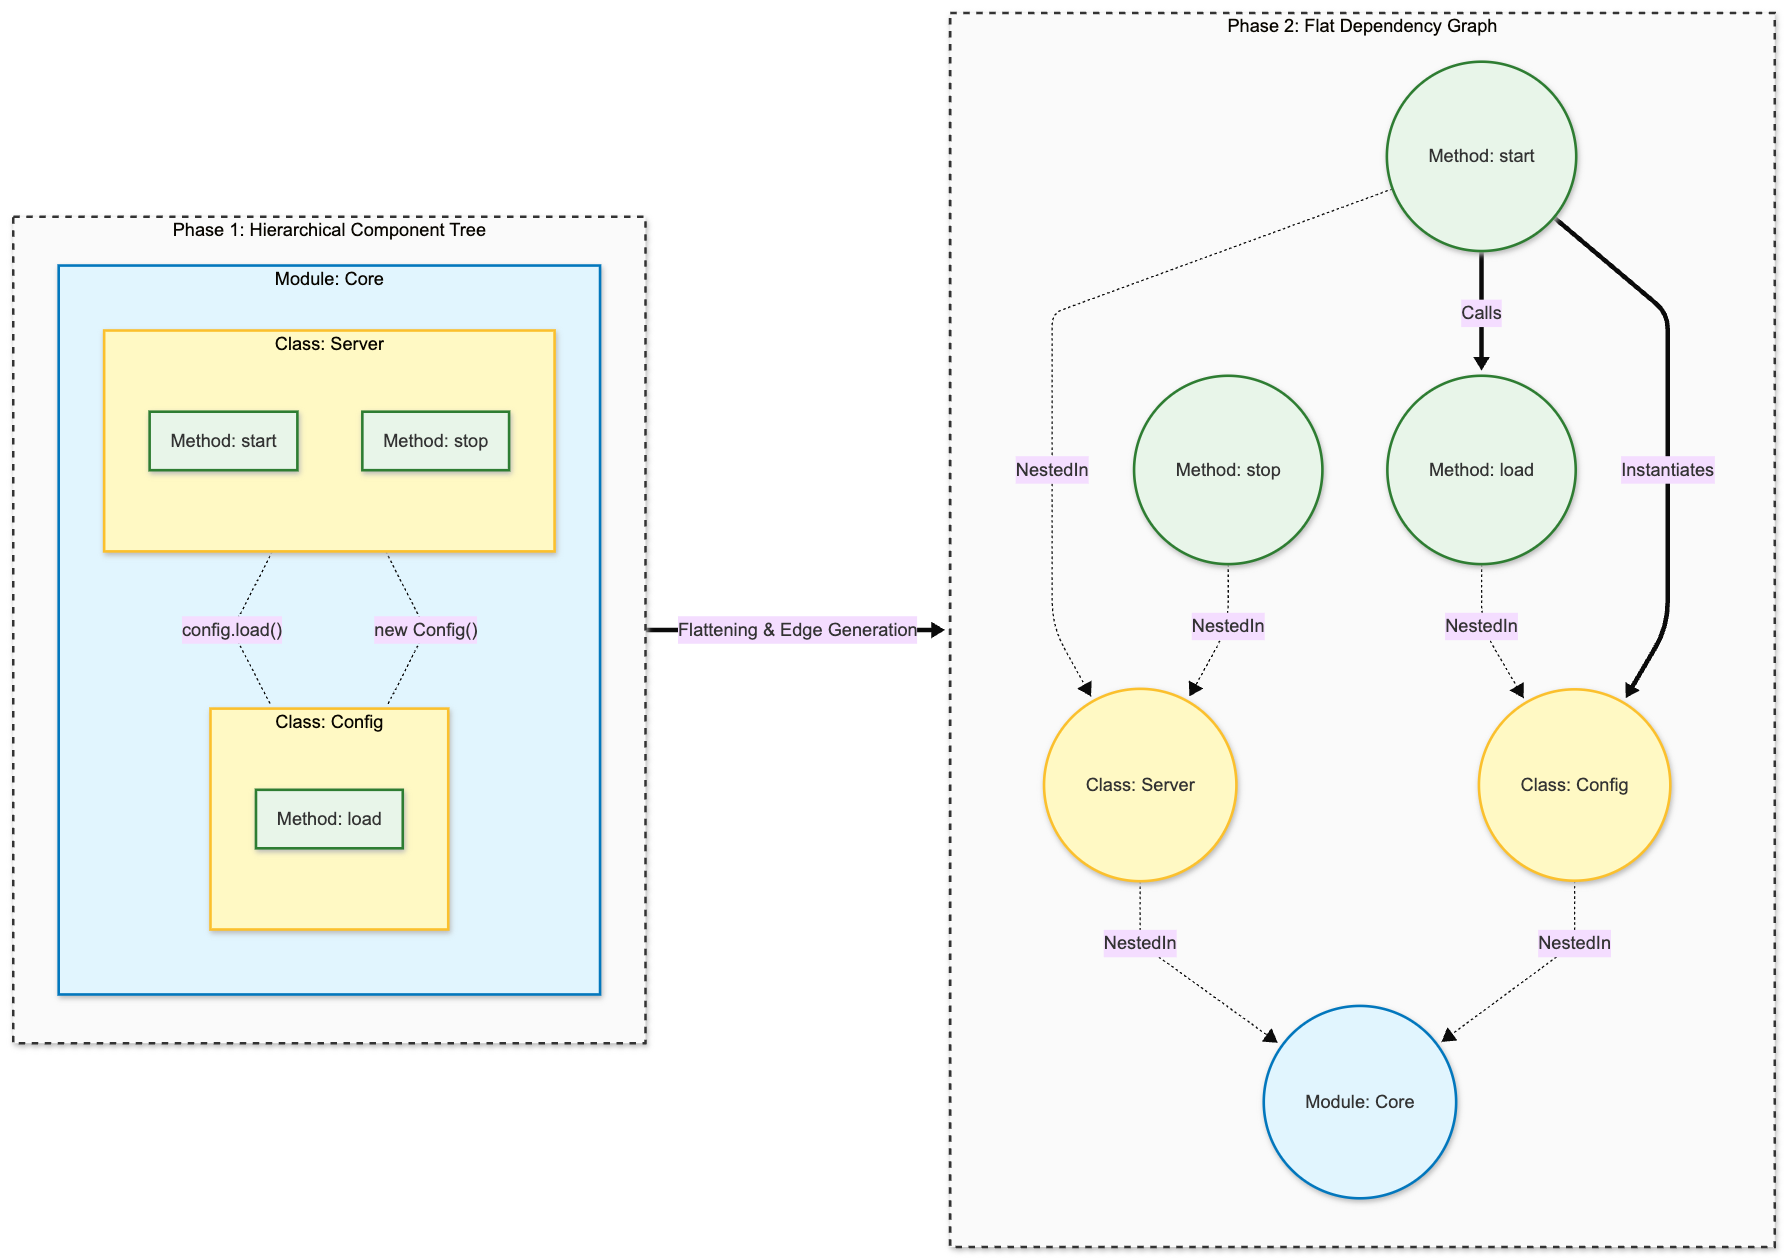
\includegraphics[width=\textwidth]{images/graph_flattening_process.png}
  \caption{Visual representation of the Component Tree flattening
    process, where nested elements are promoted to top-level graph
  nodes and hierarchical containment is converted to \textit{NestedIn} edges.}
  \label{fig:graph_flattening}
\end{figure}
